%\makeatletter
%\def\toclevel@chapter{-1}
%\makeatother

\chapter{Introduction}
%\addcontentsline{toc}{chapter}{Introduction}

Le désordre est omniprésent dans la nature, les systèmes parfaitement ordonnés étant extrêmement rares. Le désordre se manifeste sous de nombreuses formes, telles que des particules en suspension dans l'atmosphère, un agencement irrégulier des cellules dans les tissus biologiques, ou encore des impuretés dans des matériaux conducteurs. La problématique de la propagation d'ondes dans un milieu désordonné est donc une thématique générale de la physique, commune à de nombreux domaines parmi lesquels on peut citer l'imagerie en milieu opaque, la sismologie, la physique de l'atmosphère ou encore la conduction électrique. 

Que ces ondes soient de nature classique ou quantique, la description de leur propagation repose sur la notion de marche aléatoire. Au cours de leur propagation, ces ondes se heurtent à des obstacles qui changent leur trajectoire de manière aléatoire, exhibant ainsi une dynamique diffusive. La distance typique $x$ parcourue pendant un temps $t$ est alors donnée par
\begin{equation}
x\propto\sqrt{Dt} \text{ ,}
\end{equation}
avec $D$ le coefficient de diffusion. Cette description classique de la propagation repose sur le brouillage des effets d'interférence, lié à moyennage sur un grand nombre de déphasages aléatoires. La propagation de l'onde est alors considérée comme incohérente.

En s'intéressant à la diffusion cohérente d'électrons dans les solides, \emph{P.W. Anderson} a montré en 1958 que le phénomène de diffusion pouvait être annulé, $D=0$, sous certaines conditions \citep{anderson1958absence}. Anderson a ainsi révélé l'existence de conséquences macroscopiques des effets d'interférence survivant au moyennage sur les différentes réalisations du désordre. Ce phénomène commun à tout type d'onde, baptisé \emph{Localisation d'Anderson}, a depuis fait l'objet de recherches intenses, aussi bien théoriques qu'expérimentales. 


\section{Localisation d'atomes ultra-froids}

Les atomes ultra-froids constituent un outil très versatile permettant de simuler des hamiltoniens sur mesure. Ceux-ci promettent de nombreuses applications telles que les lasers à atomes \citep{robins2013atom}, des interféromètres atomiques \citep{canuel2014matter}, des horloges atomiques sur réseaux optiques \citep{derevianko2011colloquium} encore le domaine récent de l'atomtronique \citep{eckel2014hysteresis}. Ces systèmes présentent ainsi un degré de contrôle inédit des paramètres expérimentaux à l'aide de nombreux outils d'interaction matière-rayonnement \citep{bloch2012quantum}. Il est en effet possible de
\begin{itemize}
\item[\textendash] Générer des potentiels sur mesure. À l'aide d'ondes lasers, il est possible de réaliser des potentiels harmoniques, quartiques, sinusoïdaux, des potentiels désordonnés...
\item[\textendash] Contrôler les interactions entre particules. De nombreuses espèces atomiques possèdent des résonances de Feshbach, qui permet de contrôler les interactions inter-atomique à l'aide de champs magnétiques. Il est ainsi possible de générer des interactions attractives, répulsives, ou bien encore de les annuler \citep{walraven2010elements}.
\item[\textendash] Imager la fonction d'onde d'un état quantique macroscopique. Il s'agit alors d'imagerie \emph{in-situ}, souvent difficilement réalisable dans d'autres systèmes. Il est de plus possible d'obtenir une grande résolution, capable de détecter un unique atome \citep{ott2016single}.
\end{itemize}



L'observation directe de la localisation d'Anderson d'ondes de matière à une dimension en 2008 a marqué une étape importante dans l'étude de systèmes désordonnés à l'aide d'atomes ultra-froids \citep{roati2008anderson}\citep{billy2008direct}. Rapidement, les efforts se sont tournés vers l'observation de la localisation d'Anderson à trois dimensions, rapportée par trois expériences \citep{kondov2011three}\citep{jendrzejewski2012three}\citep{semeghini2015measurement} au cours de la dernière décennie. Des signatures d'effets de localisation ont par suite été recherchées dans l'espace des vitesses, menant à la mesure des paramètres microscopiques de la diffusion \citep{richard2019elastic} ainsi qu'à l'observation du pic de rétro-diffusion cohérente \citep{jendrzejewski2012coherent}, signature d'effets de localisation faible. La preuve de la cohérence des processus de localisation faible a ensuite été observée sur notre expérience en manipulant la symétrie par renversement du temps \citep{muller2015suppression}. 

Les efforts expérimentaux sont à présent tournés vers l'étude du régime critique de la transition de phase quantique d'Anderson, qui reste un véritable défi expérimental. Si les comportements localisés et diffusifs ont pu être observés dans les expériences pionnières de la localisation d'Anderson à trois dimensions, aucune n'a pu sonder le régime critique, ni même déterminer précisément l'énergie critique de la transition, appelée \emph{seuil de mobilité}. Cette étude représente l'objectif de l'équipe de recherche au sein de laquelle ma thèse s'est déroulée.

Mentionnons l'existence d'un autre système basé sur des atomes froids, le système de \emph{rotateurs forcés}, s'intéressant à la localisation dynamique, équivalent de la localisation d'Anderson dans l'espace des vitesses. Ces systèmes témoignent de résultats impressionnants: l'expérience de Lille rapporte l'observation de la localisation à trois dimensions \citep{chabe2008experimental}, l'étude du régime critique\footnote{Il s'agit de la seule expérience réalisée rapportant une mesure des exposants critiques compatibles avec les simulations numériques.} et de l'universalité de la transition d'Anderson \citep{lopez2012experimental}, ainsi que l'observation de l'analogue du pic de diffusion cohérente vers l'avant, signature de la localisation d'Anderson récemment découverte \citep{hainaut2018controlling}.


\section{Déroulement de la thèse}
%\addcontentsline{toc}{section}{Déroulement de la thèse}

\subsection{Contribution scientifique}
Les trois expériences témoignant de la localisation d'Anderson d'onde de matière à trois dimensions n'ont pas pu fournir une mesure directe du seuil de mobilité. Notamment, l'application du désordre sur l'état initial élargit significativement sa distribution d'énergie. De fait, une fraction des atomes pour lesquels $E<\Ec$ reste localisée, tandis qu'une majorité d'énergie supérieure au seuil de mobilité ont un comportement diffusif, comme illustré figure \ref{fig:AL3D}. Si l'estimation de la fraction localisée est mesurable expérimentalement, la détermination du seuil de mobilité demande une connaissance fine de la distribution d'énergie des atomes dans le désordre. En particulier, Pasek et al. ont montré de fortes déviations entre les différentes estimations expérimentales du seuil de mobilité et les estimations issues de simulations numériques \citep{pasek2017anderson}.

Dans l'optique de sonder le régime critique de la transition d'Anderson, il s'avère nécessaire de mesurer la distribution d'énergie des atomes dans le désordre, liée à la fonction spectrale \citep{pasek2017anderson}. Pour cela, l'équipe a développé une approche spectroscopique pouvant adresser sélectivement les différentes énergies du désordre, et ayant mené à la mesure des fonctions spectrales \citep{volchkov2018measurement}\citep{denechaud2018vers}. Cependant, différentes contraintes expérimentales associées à cette approche spectroscopique n'ont pas permis de procéder aux expériences d'expansion nécessaires à la mesure du seuil de mobilité.

\begin{figure}
\centering
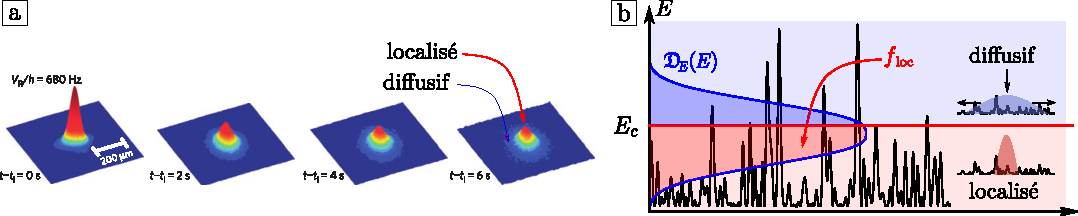
\includegraphics[width=\textwidth]{Fig/Introduction/AL3D.pdf}
\caption{\textbf{Observation de la localisation d'Anderson à trois dimensions.} \textbf{a:} images expérimentales de la localisation d'Anderson d'ondes de matière. Une partie des atomes reste localisée à temps long, tandis que le reste des atomes diffuse lentement. \textbf{b:} Illustration de la distribution d'énergie des atomes. La partie de basse énergie est localisée, tandis que la partie de haute énergie est diffusive. Ces comportements sont séparés par une transition de phase, d'énergie critique $\Ec$ appelée seuil de mobilité.}
\label{fig:AL3D}
\end{figure}

L'objectif de cette thèse était donc de dépasser les limitations expérimentales précédentes, telle qu'une limitation forte du temps de vie des atomes plongés dans le désordre, pour étendre le procédé de mesure des fonctions spectrales à la détermination du seuil de mobilité. Cependant, deux avaries majeures de l'expérience (détaillées dans la section suivante) n'ont pas rendu cette mesure possible dans le temps imparti. 

Ma contribution scientifique s'est alors focalisée sur l'exploitation des données expérimentales relatives au temps de diffusion élastique, obtenues lors de la thèse de Jérémie Richard \citep{richard2015propagation}\citep{richard2019elastic}, et leur confrontation aux mesures des fonctions spectrales \citep{signoles2019ultracold}. J'ai de plus réalisé des simulations numériques afin de compléter les mesures expérimentales, permettant de valider nos mesures du temps de diffusion élastique et de tester des modèles couramment utilisés pour la prédiction de ce dernier. Notamment, nous avons montré que l'approche des fonctions spectrales permet de décrire le comportement du temps de diffusion élastique sur la très large gamme de paramètres expérimentaux utilisée, permettant de sonder les régimes de désordre faible et de désordre fort. Cette étude nous a permis d'obtenir une vision très claire du processus de diffusion microscopique, qui constitue une brique élémentaire de la propagation d'ondes dans des milieux désordonnés.






\subsection{Contexte expérimental et déroulement de ma thèse}
%De premiers essais de stabilité du montage de désordre bichromatique, visant à dépasser la limitation du temps de vie des atomes dans le désordre identifiée lors de la mesure des fonctions spectrales, étaient en cours lors de mon arrivée à l'\emph{Institut d'Optique} en 2017. Une avarie du système informatique de contrôle de l'expérience, basé sur le logiciel \emph{Matlab}, a mis un terme à ces essais. Ce système, développé par l'ingénieur électronicien du laboratoire \emph{André Villing} parti à la retraite au cours de l'année 2017, a été remplacé par un système commercial \emph{National Instruments} et la suite \emph{Cicero Word Generator} développée au \emph{MIT} dans le groupe de \emph{Wolfgang Ketterle}. Ce remplacement, ainsi que la reconstruction de la séquence expérimentale, s'est déroulée de l'été 2017 jusqu'en mars 2018. Les changements informatiques associés ont été constants tout au long de ma thèse.
Peu après mon arrivée à l'\emph{Institut d'Optique} en 2017, un dysfonctionnement du système informatique de contrôle de l'expérience, basé sur le logiciel \emph{Matlab}, a fortement paralysé le reste de l'expérience. Ce système, développé par l'ingénieur électronicien du laboratoire \emph{André Villing} parti à la retraite au cours de l'année 2017, a été remplacé par un système commercial \emph{National Instruments} et la suite \emph{Cicero Word Generator} développée au \emph{MIT} dans le groupe de \emph{Wolfgang Ketterle}. Ce remplacement, ainsi que la reconstruction de la séquence expérimentale, s'est déroulée de l'été 2017 jusqu'en mars 2018. Les changements informatiques associés ont été constants tout au long de ma thèse. De manière plus générale, l'entièreté de l'expérience a été revue de fond en comble suite au remplacement de ce système.

\begin{figure}
\centering

\caption{\textbf{Chronologie du déroulement de ma thèse.} Stuff.}
\label{fig:chronologie_these}
\end{figure}

Au printemps 2018, une seconde avarie a paralysé l'expérience jusqu'au mois de novembre 2018. Une défaillance du circuit de refroidissement à eau des bobines de lévitation magnétique ont conduit au démontage d'une partie de l'expérience autour de la chambre de science. Des composants de génération du désordre, l'imagerie de la seconde chambre, des bobines de compensation de champs magnétiques et de lévitation ont ainsi été retirés du dispositif, puis remontés peu à peu. La calibration des champs magnétiques de la seconde chambre s'est déroulée entre le printemps et l'été 2019. L'étude du temps de diffusion élastique a eu lieu en parallèle de ces travaux de réparation, et ont duré jusqu'au printemps 2019.

Le printemps 2019 a aussi été marqué par le remplacement du laser fibré Ytterbium source pour notre piège dipolaire. La calibration de ce nouveau piège ainsi que l'optimisation de l'étape d'évaporation optique menant à la condensation de Bose-Einstein s'est déroulée jusqu'au début de l'année 2020. 

%L'entretien d'une expérience d'atomes ultra-froids nécessitant une présence quotidienne et un renouvellement constant de matériel, une mise à jour du système laser dédié au refroidissement est actuellement en cours. Nos lasers \emph{fait-maison} sont ainsi progressivement remplacés par des systèmes commerciaux \emph{Sacher Lasertechnik Cheetah}.




\section{Structure du manuscrit}
%\addcontentsline{toc}{section}{Structure du manuscrit}
Ce manuscrit se décompose selon les six chapitres suivants:
\begin{itemize}
\item[\textendash] \textbf{Chapitre \ref{ch:Localisation}: {\hypersetup{linkcolor=black}\nameref{ch:Localisation}}.} Nous commencerons par présenter les grandes lignes du transport quantique en milieu désordonné pour introduire le phénomène de localisation d'Anderson, pour ensuite nous attarder sur la transition de phase d'Anderson entre états localisés et états diffusifs. Nous nous concentrerons particulièrement sur l'état de l'art de la transition d'Anderson à l'aide des expériences d'atomes ultra-froids.  Nous ferons ainsi apparaître la quantité centrale de l'étude de la physique du désordre, la fonction spectrale. \\

\item[\textendash] \textbf{Chapitre \ref{ch:BEC_manip}: {\hypersetup{linkcolor=black}\nameref{ch:BEC_manip}}.} Dans un second temps, nous présenterons les grandes lignes de notre plateforme expérimentale. Nous rappellerons donc les principales propriétés d'un condensat de Bose-Einstein, ainsi que les différents processus d'interaction lumière-matière permettant de manipuler des atomes. Enfin, nous présenterons les différentes étapes d'un cycle expérimentales nous permettant d'obtenir un gaz quantique dégénéré. \\

\item[\textendash] \textbf{Chapitre \ref{ch:new_exp}: {\hypersetup{linkcolor=black}\nameref{ch:new_exp}}.} Après avoir présenté les différents éléments de notre expérience, nous allons nous focaliser sur les modifications apportées à notre dispositif au cours de ma thèse. En particulier, nous discuterons des deux éléments principaux de la chambre de science, la lévitation magnétique et le piège optique. Nos travaux sur ces éléments nous ont ainsi permis d'obtenir des condensats de Bose-Einstein bien meilleurs que précédemment, et de calibrer finement notre lévitation magnétique dans le but d'exploiter pleinement la dynamique de notre système. \\

\item[\textendash] \textbf{Chapitre \ref{ch:Speckle}: {\hypersetup{linkcolor=black}\nameref{ch:Speckle}}.} Après avoir présenté le dispositif générant notre onde de matière, nous décrirons notre milieu désordonné. Celui-ci est issu d'un champ de tavelures laser, ou \emph{speckle}, dont nous verrons les principales propriétés. Nous présenterons ainsi les différentes configurations de désordre que nous avons pu utiliser, et nous donnerons un aperçu de notre approche de désordre bichromatique visant à dépasser la contrainte du temps de vie limité des atomes dans le désordre à laquelle nous avons été confrontés. \\

\item[\textendash] \textbf{Chapitre \ref{ch:TauS_PRL}: {\hypersetup{linkcolor=black}\nameref{ch:TauS_PRL}}.} Ce chapitre se focalise sur la mesure du temps de diffusion élastique d'une onde de matière dans un potentiel désordonné optique. En suivant son évolution sur un large régime de paramètres, nous pourrons identifier le régime de diffusion faible pour lequel le temps de diffusion élastique est correctement décrit par l'approximation perturbative de Born. De plus, nous étudierons de manière quantitative la pertinence du critère de désordre faible $k_{\mathrm{i}}\ls^{\mathrm{Born}}=1$, et nous verrons que celui-ci dépend fortement de la nature du désordre considéré. \\

\item[\textendash] \textbf{Chapitre \ref{ch:TauS_NJP}: {\hypersetup{linkcolor=black}\nameref{ch:TauS_NJP}}.} Dans ce dernier chapitre, nous tacherons de décrire le comportement du temps de diffusion élastique à l'aide des fonctions spectrales. Nous verrons ainsi qu'une extension de l'approche perturbative ne permet pas d'étendre le domaine de validité de l'approximation de Born. De plus, nous verrons que l'approximation auto-consistante de Born, couramment utilisée, échoue à reproduire le comportement du temps de diffusion élastique dans un désordre de type \speckle . Nous verrons donc que la connaissance fine des détails de la fonction spectrale est nécessaire pour décrire la dynamique d'une onde de matière dans un désordre \speckle .
\end{itemize}


%\makeatletter
%\def\toclevel@chapter{0}
%\makeatother